\chapter{Wprowadzenie do Thread}
\label{cha:wprowadzenie}

Niniejszy rozdział ma na celu przybliżenie informacji dotyczącej Thread, poprzez przedstawienie i omówienie stosu protokołów, wyszczególnienie urządzeń i ról, w jakich pracują węzły sieci Thread oraz zaprezentowanie wybranych, podstawowych mechanizmów, przydatnych do zrozumienia zagadnienia sieci Thread. Rozważania w poniższym rozdziale oparte zostały o publiczną dokumentację Thread \cite{thread-1.3.0}.

\section{Stos protokołów}
\label{sec:thread-stack}

    Stos protokołów Thread obejmuje warstwę sieciową oraz transportową Modelu OSI (ang. \textit{ISO Open Systems Interconnection Reference Model}) i jest dedykowany dla urządzeń opartych o warstwę fizyczną oraz warstwę łącza danych standardu IEEE 802.15.4. Na Rysunku \ref{fig:thread-sprotocol-stack}. przedstawiono warstwy Thread oraz wdrożone w nich protokoły komunikacyjne.

    \begin{figure}[H]
        \centering
        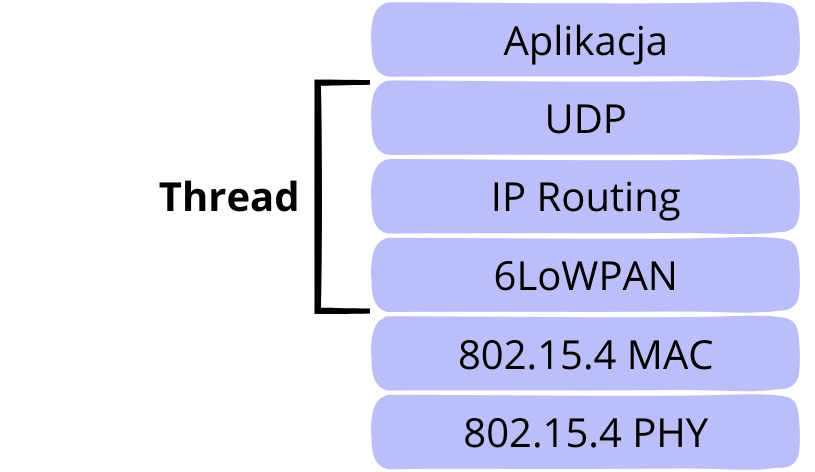
\includegraphics[width=0.8\linewidth]{graphics/thread-protocol-stack.png}
        \caption{Stos protokołów Thread.}
        \label{fig:thread-sprotocol-stack}
    \end{figure}

    \subsection{Warstwa Fizyczna oraz Warstwa Łącza Danych}

        Protokół Thread jest stworzony dla urządzeń, których 2 pierwsze warstwy modelu OSI są oparte o standard definiujący LR-WPAN w wersjach IEEE 802.15.4-2006 lub IEEE 802.15.4-2015. Jednakże nie jest wymagane, aby urządzenia Thread funkcjonowały w sieciach LR-WPAN. Ponadto protokół Thread nie wykorzystuje zdefiniowanych w IEEE 802.15.4 ról, takich jak:
        \begin{itemize}
            \item FFD (ang. \textit{Full-Function Device}),
            \item RFD (ang. \textit{Reduced-Function Device}),
            \item Koordynatora PAN (ang. \textit{Personal Area Network Coordinator}).
        \end{itemize}

    \subsection{Warstwa Sieciowa}

        W warstwie 3. Modelu OSI Thread implementuje protokół IPv6.
        
        W celu umożliwienia przesyłania pakietów IPv6 nad LR-WPAN wprowadzono warstwę adaptacyjną 6LoWPAN. Usprawnienie to pozwala na enkapsulacje pakietów IPv6 do IEEE 802.15.4 MSDU (ang. \textit{MAC Service Data Unit}) oraz definiuje mechanizmy kompresji nagłówków IPv6, fragmentacji i składania pakietów IPv6, odpowiednio do oraz z IEEE 802.15.4 MSDU.
        
        Do trasowania (ang. \textit{routing}) Thread wykorzystuje zdefiniowany w rozdziale 5.9 dokumentacji \cite{thread-1.3.0} protokół rutingu typu distance vector.

    \subsection{Warstwa Transportowa}
    
        Do komunikacji między węzłami w warstwie transportowej sieć Thread używa UDP (ang. \textit{User Datagram Protocol}). Protokół ten jest wymagany przy implementacji stosu Thread, ponieważ jest wykorzystywany w procesach sygnalizacyjnych oraz mechanizmach zarządzania siecią Thread.
    
        Wdrożenie TCP (ang. \textit{Transport Control Protocol}) nie jest obligatoryjne. Natomiast w przypadku potrzeby uwzględnienia TCP, Thread definiuje wskazówki do efektywnej implementacji tego protokołu w rozdziale 6.2 dokumentacji \cite{thread-1.3.0}.

\section{Typy urządzeń oraz role}
\label{sec:device-types}

    Niniejsza sekcja ma na celu objaśnienie podstawowych ról węzłów w sieci Thread oraz terminologii, wykorzystywanej w opisywaniu mechanizmów sieci.

    \subsection{Podstawowe role urządzeń}

    W celu pełnej klasyfikacji węzłów w sieci Thread dokonano ich podziału ze względu na umiejętność przekazywania (ang. \textit{forwarding}) pakietów oraz opisano ich charakterystykę:
    \begin{enumerate}
        \item Ruter (ang. \textit{router}):
        \begin{itemize}
            \item posiada możliwość przekazywania pakietów między węzłami sieci,
            \item odbiornik urządzenia pozostaje włączony cały czas,
            \item jest niezbędnym elementem w procesie dołączania innego urządzenia do sieci Thread.
        \end{itemize}
        \item Urządzenie końcowe, ED (ang. \textit{End Device}):
        \begin{itemize}
            \item nie posiada możliwości przekazywania pakietów do innych węzłów,
            \item może komunikować się bezpośrednio tylko z sąsiadującym Ruterem,
            \item odbiornik urządzenia może zostać wyłączony w celu ograniczenia zużycia mocy.
        \end{itemize}
    \end{enumerate}

    ED, stanowiące rolę \textit{Dziecka} (ang. \textit{Child}), pozostaje zawsze połączone z wyłącznie jednym Ruterem, którego określa się terminem \textit{Rodzic} (ang. \textit{Parent} lub \textit{Parent Router}).

    \subsection{Typy urządzeń}
    \label{subsec:device-types}

        Ostatecznie, dokonano podziału urządzeń Thread, wyszczególniając dwa główne typy:
        \begin{enumerate}
            \item FTD (ang. \textit{Full Thread Device}),
            \item MTD (ang. \textit{Minimal Thread Device}).
        \end{enumerate}

        Pełną klasyfikację urządzeń w sieci Thread, z kryterium podziału ze względu na typ, przedstawiono na Rys \ref{fig:thread-device-taxonomy}.

        \subsubsection{Full Thread Device}

            FTD mogą funkcjonować w sieci zarówno w roli Urządzeń Końcowych, jak i w roli Ruterów. Dalej można wyszczególnić: 
            \begin{itemize}
                \item Ruter (ang. \textit{Router}) - urządzenie pełniące wspomnianą rolę Rutera.
                \item REED (ang. \textit{Router Eligible End Device}) - rodzaj Urządzenia Końcowego, które może zostać awansowane do roli Rutera.
                \item FED (ang. \textit{Full End Device}) - rodzaj Urządzenia Końcowego, które nie może zostać awansowane do roli Rutera.
            \end{itemize}
        
        \subsubsection{Minimal Thread Device}

            MTD ograniczone są jedynie do pełnienia roli Urządzeń Końcowych. Kolejno można wyróżnić:
            \begin{itemize}
                \item MED (ang. \textit{Minimal End Device}) - rodzaj Urządzenia Końcowego, którego odbiornik jest zawsze włączony.
                \item SED (ang. \textit{Sleepy End Device}) - rodzaj Urządzenia Końcowego, którego odbiornik jest wyłączony przez większość czasu, natomiast włącza się okazjonalnie, aby odebrać pakiety przekazane przez Rodzica.
            \end{itemize}

        \begin{figure}[H]
            \centering
            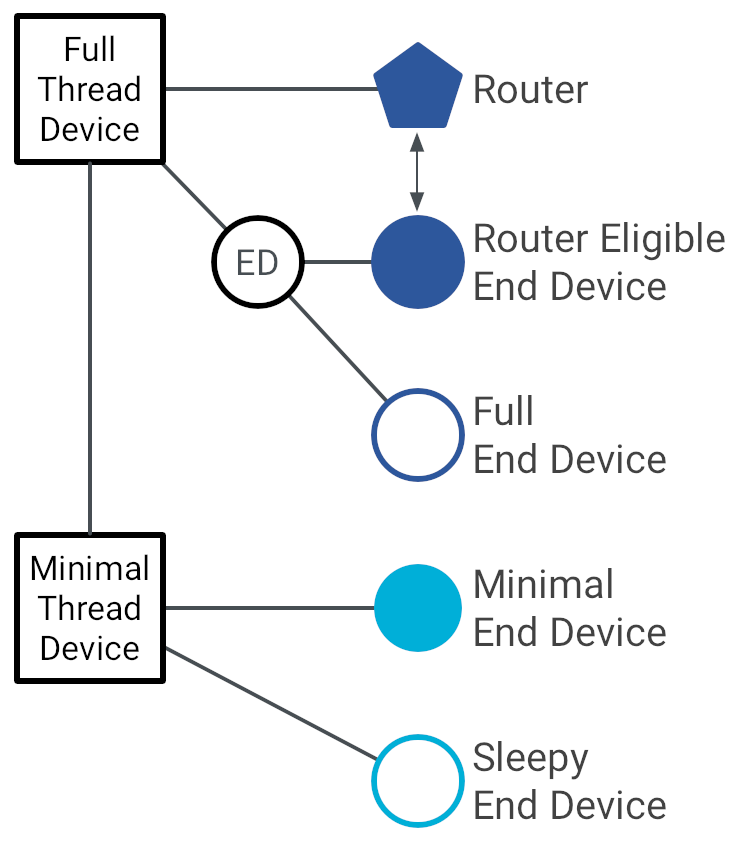
\includegraphics[width=0.8\linewidth]{graphics/external/ot-primer-taxonomy.png}
            \caption{Podział urządzeń w sieci Thread ze względu na typ \cite{ot-devices}.}
            \label{fig:thread-device-taxonomy}
        \end{figure}

    \subsection{Dodatkowe role Rutera}

        Poza podstawową funkcjonalnością, jaką jest przekazywanie pakietów między węzłami sieci, Ruter w sieci Thread może posiadać dodatkowe role. Między innymi są to:
        \begin{itemize}
            \item Lider (ang. \textit{Leader}),
            \item Ruter Brzegowy (ang. \textit{Border Router}).
        \end{itemize}

        \subsubsection{Lider}

        Topologia sieci Thread jest dynamiczna i role poszczególnych węzłów zmieniają się w czasie. Za mechanizm awansu ED do Ruterów oraz degradacji Ruterów do ED odpowiada Ruter pełniący rolę Lidera. Opisane zachowanie jest istotne w momencie wystąpienia awarii, gdy jeden z węzłów nie może pełnić swojej roli. Taka cecha sieci nazywana jest samoleczeniem (ang. \textit{self-healing}) i jest charakterystyczna dla sieci kratowych Thread.

        Główne funkcje Lidera:
        \begin{itemize}
            \item Awans do Ruterów oraz ich degradacja poprzez zarządzanie numerem ID Rutera (ang. \textit{Router ID}),
            \item Zbierania i rozsyłanie informacji o sieci Thread.
        \end{itemize}

        Proces awansu i degradacji węzłów przez Lidera uwzględnia możliwości typów urządzeń opisane w podsekcji \ref{subsec:device-types}. W jednej sieci Thread rolę Lidera może pełnić tylko jedno urządzenia. W momencie tworzenia topologii, urządzenie FTD inicjujące sieć zostaje wybierane na Lidera.
        
        \subsubsection{Ruter Brzegowy}

        W celu nawiązania komunikacji między siecią Thread a siecią IP spoza tej domeny, np. Ethernet lub IEEE 802.11, niezbędne jest, aby w sieci przynajmniej jeden Ruter funkcjonował jako Ruter Brzegowy. Posiada on minimum 2 interfejsy sieciowe - jeden interfejs sieciowy Thread oraz drugi zewnętrzny oparty o IP, najczęściej Ethernet lub WLAN (ang. \textit{Wireless Local Area Network}). Zadaniem takiego Routera jest przekazywanie pakietów IPv6 pomiędzy tymi interfejsami.

    Wymienione role Rutera mogą się nakładać. Jeden węzeł może być jednocześnie np. Ruterem Brzegowym, Liderem oraz Rodzicem dla innego ED.

\section{Przegląd wybranych mechanizmów sieci Thread}

    \subsection{Tworzenie sieci}
    \label{subsec:network-forming}

    Formowanie sieci Thread rozpoczyna się od wybrania numeru kanału (ang. \textit{channel}) oraz identyfikatora PAN ID (ang. \textit{Personal Area Network Identifier}) zgodnie z IEEE 802.15.4. Kolejno, aby stworzyć sieć, urządzenie inicjujące jest zobligowane do wybrania wartości poniższych parametrów:
    \begin{itemize}
        \item \textit{Thread Network Short PAN Identifier (PAN ID)} - 16 bitowa liczba całkowita bez znaku, unikalna w zasięgu skanowania.
        \item \textit{Network Key} - 16 B, do zastosowań kryptograficznych.
        \item \textit{Commissioning Credential} - 8-255 B, ciąg znaków, wykorzystywany do tworzenia klucza PSKc podczas procesu Commissioning.
        \item \textit{Mesh-Local Prefix} - prefix IPv6, wykorzystywany do adresacji urządzeń w sieci Thread.
        \item \textit{Extended PAN ID} - 8 B, identyfikuje sieć Thread w zasięgu.
        \item \textit{Network Name} - 1-16 B, ciąg znaków, identyfikuje sieć Thread.
    \end{itemize}{}

    Urządzenie inicjujące sieć zostaje Ruterem, wybierając dla siebie identyfikator \textit{RouterId}, a w konsekwencji braku innych Ruterów w sieci, zostaje również Liderem.

    \subsection{Commissioning}
    \label{subsec:commissioning}

    Commissioning to proces pozwalający nowym urządzeniom na dołączenie do istniejącej sieci Thread. W celu zapewnienia bezpieczeństwa oraz powstrzymanie niechcianych urządzeń (ang. \textit{Rouge Device}) przed połączeniem z siecią Thread węzły powinny zostać uwierzytelnione i autoryzowane. Podstawą działania mechanizmu jest protokół DTLS (ang. \textit{Datagram Transport Layer Security}).

    Do opisania mechanizmu Commissioning wprowadzono następujące terminy:
    \begin{itemize}
        \item \textit{Joiner} - rola nowego urządzenia próbującego podłączyć się do sieci.
        \item \textit{Commissioner} - rola urządzenia, który uwierzytelnia węzeł o roli Joiner.
        \item \textit{Joiner Router} - rola urządzenia, który jest Ruterem i znajduje się najbliżej sieci, do której stara się przyłączyć Joiner.
    \end{itemize}

    Ze względu na to czy Commissioner znajduje się w sieci Thread lub poza nią, wyróżniamy kolejno 2 typy procesu Commissioning \cite{thread-commissioning}:
    \begin{enumerate}
        \item \textit{On-mesh},
        \item \textit{External}.
    \end{enumerate}

    W aktualnej sekcji opisany zostanie jedynie scenariusz On-mesh, w którym Commissioner jest częścią sieci w domenie Thread.

    Na Rysunku \ref{fig:thread-on-mesh-commissioning} przedstawiono przykładową sieć Thread z wyszczególnieniem ról charakterystycznych dla procesu On-mesh Commissioning.

    W sieci Thread, w jednym momencie może istnieć dokładnie jeden Commissioner. Urządzenia, które mogą pełnić rolę Commissioner, wymieniają wiadomości z Liderem, w celu ustalenia, który z kandydatów będzie pełnił tę funkcję. Proces ten określono nazwą \textit{Petitioning}.

    Po elekcji urządzenia, który będzie pełnił rolę Commissioner, kolejne urządzenia Joiner są w stanie rozpocząć próbę dołączenia do sieci, nazwaną \textit{Joining}.
    W kolejnym kroku zestawione zostaje połączenie \\ Joiner-Joiner Router, a następnie Joiner-Commissioner, które jest zabezpieczone z użyciem protokołu DTLS ,\\ i do którego zestawienia niezbędne jest podanie przez Joinera Joining Device Credential (PSKd). Następnie Joiner zostaje uwierzytelniony na skutek wymiany kolejnych wiadomości z Commissioner. W wyniku poprawnie przeprowadzonego procesu Commissioning urządzenie posiada wszystkie niezbędne informacje, aby podłączyć się do sieci.

    \begin{figure}[H]
        \centering
        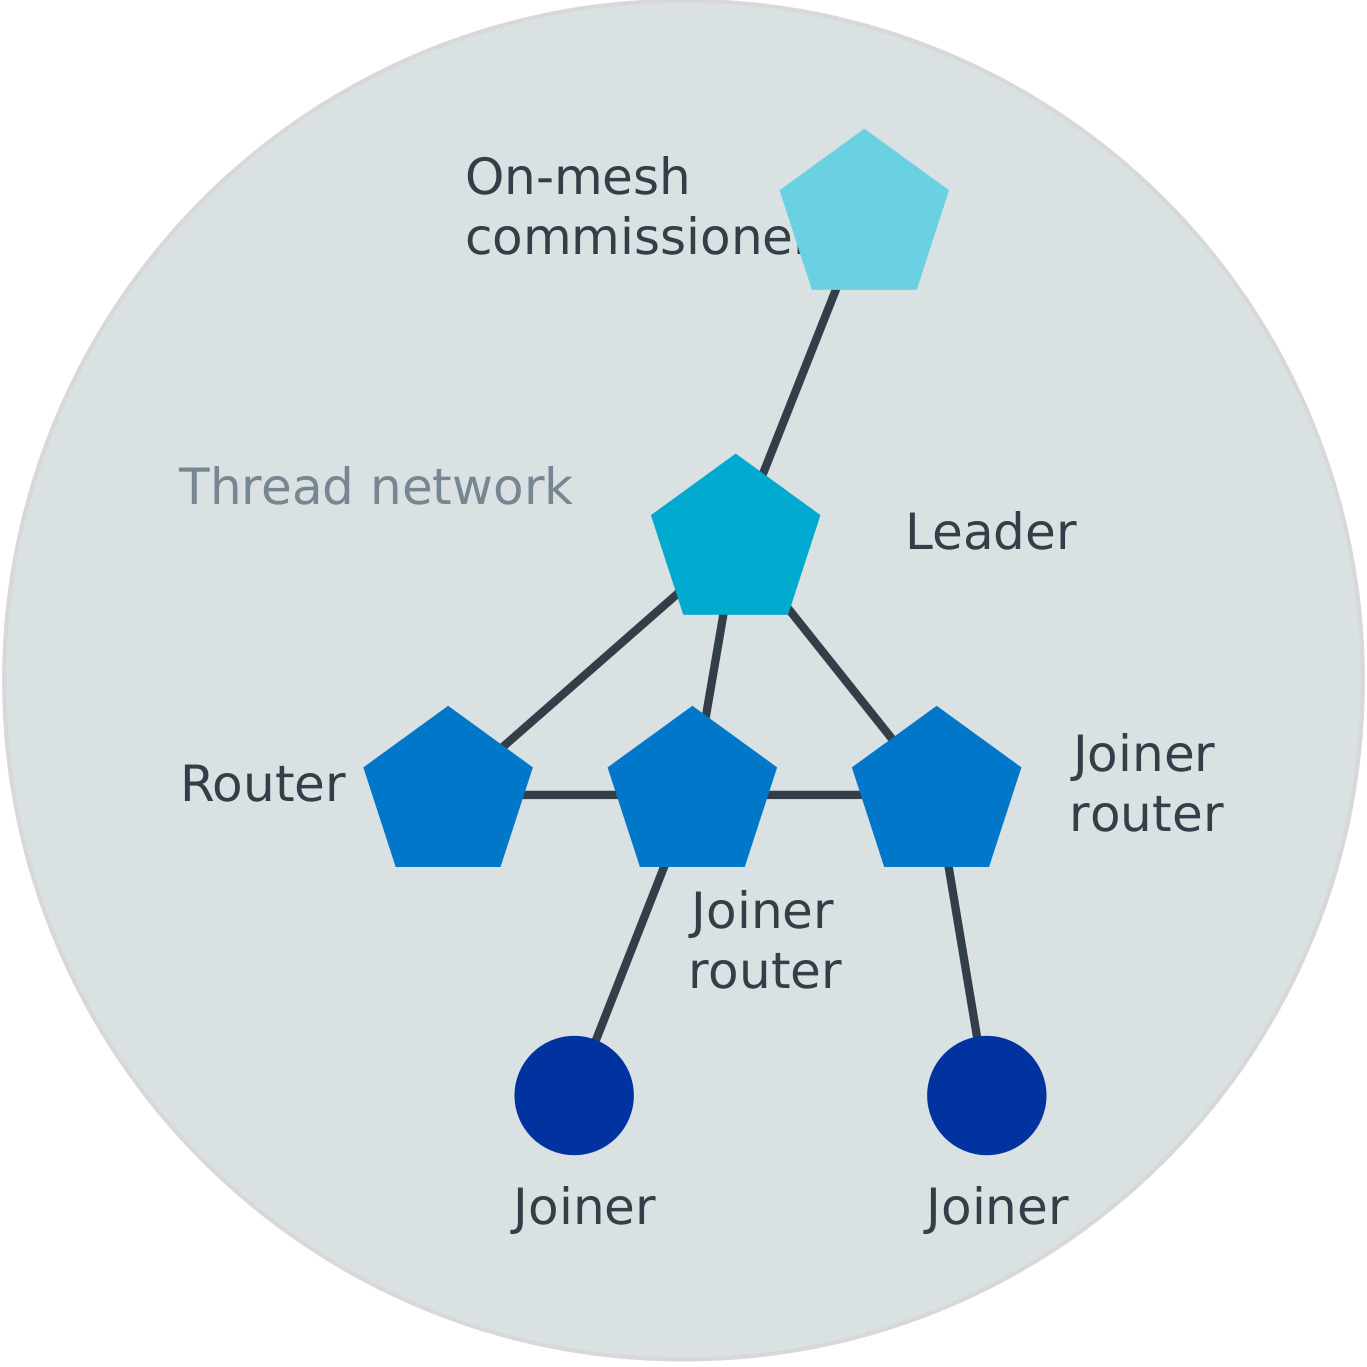
\includegraphics[width=0.8\linewidth]{graphics/external/Thread_on-mesh_commissioning.jpg}
        \caption{Przykładowa topologia sieci Thread podczas procesu On-mesh Commissioning \cite{thread-commissioning}.}
        \label{fig:thread-on-mesh-commissioning}
    \end{figure}

    \subsection{Dołączanie do sieci}

    Proces dołączania do sieci Thread rozpoczyna się od skanowania istniejących sieci IEEE 802.15.4 na kolejnych kanałach. Urządzenie podłączające się rozgłasza żądanie Beacon Request. W przypadku otrzymania wiadomości przez Rutery lub REED odpowiadają one poprzez wysłanie Beacon, który zawiera podstawowe informacje na temat danej sieci.

    Po zakończeniu procesu odkrywania sieci Thread urządzenie może próbować podłączyć się do istniejącej sieci lub utworzyć własną.

    Aby urządzenie było w stanie dołączyć do sieci Thread, jest zobowiązane do pozyskania poniższych parametrów opisujących konkretną sieć Thread:
    \begin{itemize}
        \item Network Key,
        \item PSKc,
        \item Mesh-Local Prefix,
        \item Extended PAN ID,
        \item Network Name.
    \end{itemize}
    
    Informacje te mogą zostać uzyskane w wyniku pomyślnego zakończenia procesu Commissioning.

    Urządzenie posiadające wszystkie niezbędne informacje o sieci, w kolejnym kroku zestawia połączenie Dziecko-Rodzic z wykorzystaniem mechanizmu MLE (ang. \textit{Mesh Link Establishment}). Ostatecznie, nawiązanie połączenia zakończone jest przesłaniem przez Rodzica identyfikatora Child ID. Od tego momentu urządzenie dołączające jest częścią sieci Thread.
















